\subsection{Algèbre linéaire creuse}
\`{A} la différence de l'algèbre linéaire dense, la majorité des calculs faits en creux sont irréguliers.
%
C'est en partie dû à la façon de stocker la matrice creuse.
%
En effet, pour avoir un stockage efficace, seul les coefficients non nuls de la matrice creuse sont stockés.
%
Le motif des valeurs non nulles de la matrice est définit par le problème que nous souhaitons résoudre.
%
Le format le plus générique pour stocker des matrices creuses s'appelle COO (fig.~\ref{fig:COO}).
%
Dans ce format, chaque valeur non nulles est stocké avec ses coordonnées 2D dans la matrice.
%
Une autre format, lui aussi générique, est souvent utilisé, il s'agit du format CSR\footnote{Compress Sparse Row} (fig.~\ref{fig:CSR}).
%
Les éléments non nuls sont triés par ligne puis le tableau {\em PTR} du format de stockage nous permet de retrouver la ligne d'un élément.
%
D'autre formats moins génériques existent mais nous n'en parlerons pas ici.

\begin{figure}[!ht]
     \begin{center}
        \subfigure[Exemple de matrice creuse]{%
            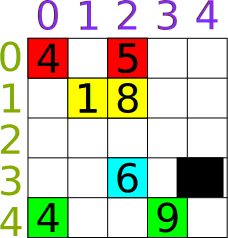
\includegraphics[width=0.25\textwidth]{matrix_format}
        }%
        \subfigure[Stockage COO]{%
           \label{fig:COO}
           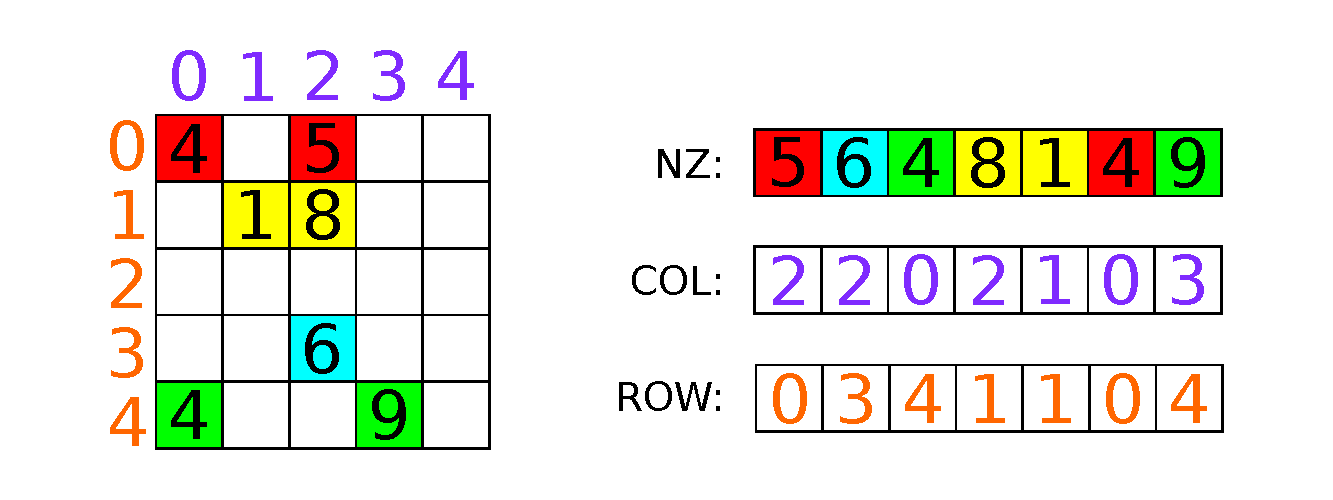
\includegraphics[width=0.35\textwidth]{COO}
        }%
        \subfigure[Stockage CSR]{%
            \label{fig:CSR}
            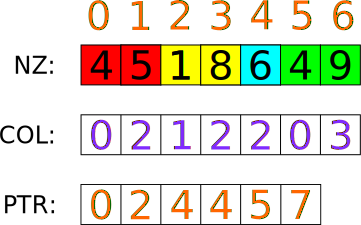
\includegraphics[width=0.35\textwidth]{CSR}
        }%
    \end{center}
    \caption{Comparaison entre les formats de stockage de matrices creuses COO and CSR.}
    \label{fig:matrix_storage}
\end{figure}

Le choix du format de stockage va avoir beaucoup d'effet sur les performances d'une application.
%
Avec la plupart des format, nous aurons au moins deux accès mémoire pour obtenir les coordonnées 2D d'un coefficient non nul alors qu'avec l'algèbre linéaire dense nous pouvons calculer ces coordonnées à partir de la position dans la matrice.
%
Une partie non négligeable de la bande passante mémoire est utilisée juste pour les coordonnées 2D.
%
Les propriétés creuse et irrégulière de ces matrices impliquent aussi une mauvaise efficacité mémoire des noyaux d'algèbre linéaire creux à cause d'une mauvaise réutilisation du cache.
%
La plupart des optimisations faites en algèbre linéaire dense ne peuvent pas être appliquées à l'algèbre linéaire creuse à cause de l'irrégularité dans l'ordre des calculs ainsi que dans les accès mémoire.
%
Mais l'algèbre linéaire creuse nous permet de résoudre des problèmes bien plus grands que ceux qui utilisent l'algèbre linéaire dense.
%
Ceci est dû au fait qu'avec une taille de matrice équivalente, l'algèbre linéaire creuse utilise vraiment moins de mémoire que l'algèbre linéaire dense.


Résoudre des problèmes linéaires creux est aussi très différent de résoudre des problèmes denses.
%
Nous ne pouvons pas utiliser une inversion directe de matrice, ou la technique de l'élimination de Gauss parce que nous obtiendrions une matrice quasi-dense.
%
Or une matrice quasi-dense avec de grandes dimensions ne pourrait pas tenir en mémoire et même si c'était le cas, le nombre de calculs serait trop important.
%
Donc des méthodes différentes ont été inventées pour être capable de résoudre ces problèmes, beaucoup sont basées sur des méthodes itératives.
%
Nous démarrons donc avec une solution, ensuite ces algorithmes réduisent itérativement la différence entre notre solution approximée et la solution réelle.
%
\`{A} la fin, nous obtenons une bonne approximation de la solution, ce qui est souvent suffisant pour être considérée comme la solution au problème.
